\chapter{Planung}

\section{Problemstellung}

Ziel des Echtzeitsysteme Praktikums war es eine Grill Simulation
zu entwickeln. Das Hauptaugenmerk der Simulation lag auf den Grillwürsten, die von
verschiedenen Prozessen behandelt werden. Diese Prozesse sind teilweise
physikalischer Natur (z.B. das Bräunen), teilweise handelt es sich auch um „Akteure“
(Fleischer, Grillmeister und Feuerwehr). Jeder dieser natürlichen Prozesse wird in der
Simulation auf einen Task abgebildet. Dort, wo die natürlichen Prozesse Informationen
und Gegenstände austauschen, werden die Tasks entsprechende Daten austauschen.
Diese Kommunikation zwischen den Tasks ist Kern dieser Aufgabe!
Jede Wurst durchläuft während der Simulation mehrere Stationen an denen sie von
den unterschiedlichen Prozessen behandelt wird. Nach ihrer Erzeugung durch den
Fleischer liegt die Wurst in einer Kühlbox. Dort verbleibt sie so lange, bis sie durch
Eingreifen des Benutzers entnommen und dem Grillmeister übergeben wird. Der
Grillmeister platziert die Wurst auf dem Grill. Die Wurst wird nun von einer Seite
gebräunt (sie hat insgesamt vier zu bräunende Seiten), bis sie vom Grillmeister
gedreht oder entfernt wird. Wenn eine Wurst von einer Seite zu lange gebräunt wird,
platzt sie und entzündet den Grill. Der Grill kann nur von der Feuerwehr gelöscht
werden.

\section{Analyse}

\subsection{Tasks}

Aus der Problemstellung lassen sich folgende, als Tasks zu modellierende, Programmteile identifizieren.

\begin{itemize}
\item Fleischer (Produziert Würste)
\item Grillmeister (Verwaltet die auf dem Grill befindlichen Würste)
\item Feuerwehr (Prüft und löscht den Grill)
\item Physik (Bräunt Würste und entzündet den Grill)
\item Eingabe (Abarbeiten von Benutzereingaben)
\item Ausgabe (Gibt den Status der Grill-Simulation aus)
\end{itemize}

Die Prioritäten wurden nach Analyse der Aufgabestellung so angepasst, dass sich die Tasks nicht unnötig blockieren und jeder Task die Chance hat vom Scheduler erfasst zu werden.
Zudem wurden Ein- und Ausgabe so priorisiert, dass Eingaben schnell erkannt werden und die Ausgabe den Rest der Simulation nicht blockiert.

\subsection{Prozesskommunikation}

Damit Tasks untereinander Kommunizieren können müssen Kommunikationsdienste eingerichtet werden, die andere Tasks nicht blockieren und den reibungslosen Ablauf der Simulation gewährleisten.

\subsubsection{Kühlbox}

Die Kühlbox soll von dem Fleischer-Task befüllt und von dem Grillmeister-Task geleert werden.
Hierfür eignet sich eine Nachrichten-Warteschlange, da hier nur Objekte (Würste) rein- und rausgenommen werden
und keine größeren kritische Abschnitte entstehen.
Im Gegensatz zur Semaphor können in der Warteschlange direkt Objekte hinterlegt werden und eine zusätzliche Datenstruktur kann vermieden werden.

\subsubsection{Grill}

Der Grill wird permanent vom Grillmeister-, Physik und Feuerwehr-Task auf verschiedene Parameter und einzelne Würste abgefragt und verändert.
Hier wurde eine durch ein Mutex-Semaphor abgesicherte Datenstruktur geplant, da hier größere kritische Abschnitte,
wie das sequentielle Bräunen aller Würste, entstehen.

\subsubsection{Fleischer und Grillmeister}

Um die Benutzereingabe zu realisieren müssen Fleischer und Grillmeister vom Eingabe-Task aus gesteuert werden können.

Die erste Überlegung, die Kommunikation über Semaphore zu realisieren, wurde nach kurzer Evaluation verworfen.
Hierfür hätten zusätzlich Semaphore zum Absichern der Zustände von Fleischer und Grillmeister eingeführt werden müssen,
die die Komplexität syntaktisch als auch semantisch drastisch erhöht und die Erweiterbarkeit beschränkt hätten.

Da der Nachrichtenaustausch nur jeweils in Richtung Fleischer- und Grillmeister-Task geschehen muss,
wurde jeweils eine Nachrichten-Box pro Task angestrebt um so die Nutzereingabe durch versenden von Nachrichten abzubilden.

\subsection{Zusammenfassung}

Nach Analyse der Problemstellung wurde ein Diagramm zur Visualisierung der Prozesskommunikation, inklusive der zu verwendenden Kommunikationsdienste, erstellt.

\begin{figure}[!ht]
  \centering
  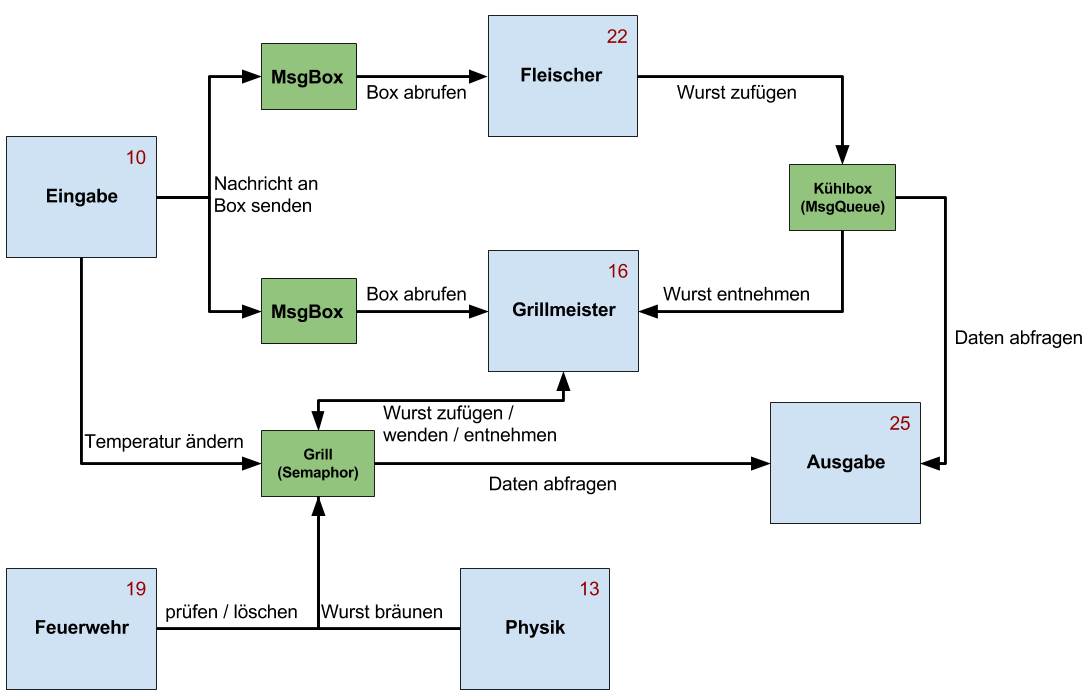
\includegraphics[width=\textwidth]{Bilder/diagramm_ipc.png}
  \caption{IPC}
\end{figure}
